\documentclass[12pt,letterpaper]{article}
\usepackage[latin1]{inputenc}
\usepackage{amsmath}
\usepackage{amsfonts}
\usepackage{amssymb}
\usepackage{setspace}
\usepackage{graphicx}
\usepackage{epsfig}
\usepackage{booktabs}
\graphicspath{{./images/}} % Figures path - used in graphicx
\author{Christopher C. Lamb}
\title{Policy-centric Overlay Networks for Usage Management}

\date{\today}
\begin{document}

\maketitle

\doublespacing

\begin{abstract}
Overlay networks have become a widely used technology with examples ranging from consumer focused distribution systems like BitTorrent to commercial content distribution systems like Akamai.  These kinds of systems, with the appropriate policy-centric content management components, can address looming problems in information distribution that both companies and federal agencies are beginning to face with respect to sensitive content.  This work addresses the current state of the art in these kinds of systems, reviewing current example system architectures from the Unified Cross Domain Management Office (UCDMO), a federal organization specifically tasked with addressing these issues.  It then covers other related work, introduces a taxonomy of types of policy-centric usage managed network systems, and proposes specific work that represents a significant contribution to the understanding of such systems. 
\end{abstract}

\section{Introduction}
Current enterprise computing systems are facing a troubling future.  As things stand today, they are too expensive, unreliable, and information dissemination procedures are just too slow.

Generally, such systems still do not use current commercial resources as well as they could and use costly data partitioning schemes.  Most of these kinds of systems use some combination of systems managed in house by the enterprise itself rather than exploiting lower cost cloud-enabled services.  Furthermore, many of these systems have large maintenance loads imposed on them as a result of internal infrastructural requirements like data and database management or systems administration.  In many cases networks containing sensitive data are separated from other internal networks to enhance data security at the expense of productivity, leading to decreased working efficiencies and increased costs.

These kinds of large distributed systems suffer from a lack of stability and reliability as a direct result of their inflated provisioning and support costs.  Simply put, the large cost and effort burden of these systems precludes the ability to implement the appropriate redundancy and fault tolerance in any but the absolutely most critical systems.  Justifying the costs associated with standard reliability practices like diverse entry or geographically separated hot spares is more and more difficult to do unless forced by draconian legal policy or similarly dire business conditions.

Finally, the length of time between when a sensitive document or other type of data artifact is requested and when it can be delivered to a requester with acceptable need to view that artifact is prohibitively long.  These kinds of sensitive artifacts, usually maintained on partitioned networks or systems, require large amounts of review by specially trained reviewers prior to release to data requesters.  In cases where acquisition of this data is under hard time constraints like sudden market shifts or other unexpected conditional changes this long review time can result in consequences ranging from financial losses to loss of life.

Federal computer systems are prime examples of these kinds of problematic distributed systems, and demonstrate the difficulty inherent in implementing new technical solutions.  They, like other similar systems, need to be re-imagined to take advantage of radical market shifts in computational provisioning.

\section{Motivation}
Current policy-centric systems are being forced to move to cloud environments and incorporate much more open systems.  Some of these environments will be private or hybrid cloud systems, where private clouds are infrastructure that is completely run and operated by a single organization for use and provisioning, while hybrid clouds are combinations of private and public cloud systems.  Driven by both cost savings and efficiency requirements, this migration will result in a loss of control of computing resources by involved organizations as they attempt to exploit economies of scale and utility computing.

Robust usage management will become an even more important issue in these environments.  Federal organizations poised to benefit from this migration include agencies like the National Security Agency (NSA) and the Department of Defense (DoD), both of whom have large installed bases of compartmentalized and classified data.  The DoD realizes the scope of this effort, understanding that such technical change must incorporate effectively sharing needed data with other federal agencies, foreign governments, and international organizations \cite{proposal:info-sharing-strategy}.  Likewise, the NSA is focused on exploiting cloud-centric systems to facilitate information dissemination and sharing \cite{proposal:nsa-cloud}.

Cloud systems certainly exhibit economic incentives for use, providing cost savings and flexibility, but they also have distinct disadvantages as well.  Specifically, the are not intrinsically as private as some current systems, generally can be less secure than department-level solutions, and have the kinds of trust issues that the best of therapists cannot adequately address \cite{proposal:privacy-security-trust-cloud}.

To begin with, cloud technology is not currently as private as some organizations would like:
\begin{itemize}
\item \textit{User Data Control} --- In virtually any given Software-as-a-Service (SaaS) scenario, user data controls are sadly lacking.  Once data has been committed to a specific provider, that data is completely out of the original data owners control.  Furthermore, as we will see below, that data my not even be solely owned by the original owner anymore either.
\item \textit{Secondary Use} --- Most consumer facing social systems extensively mine user provided data for additional business advantages.  This is a common and well known secondary use for supplied data.  SaaS providers again have strong incentives to examine user provided information.
\item \textit{Offshore Development} --- Service users have no real control over who actually develops the systems a given service deploys.  Organizations have attempted to contractually limit development and support functions companies pursue to, say, the continental United States but have had very poor results with these kinds of unsupportable arrangements.
\item \textit{Data Routing} --- Both system providers and system users in fact have little control over routing issues.  Prohibiting data routing through sensitive countries is a difficult task for a single organization.
\item \textit{Secondary Storage} --- Most large-scale systems expect to use Content Delivery Networks (CDNs) to help manage content, and that expectation is heavily reflected in their physical system architectures. They simply cannot divorce use of CDNs from their systems for a single organization.
\item \textit{Bankruptcy and Data Ownership} --- Ownership and obligation to maintain expected data arrangements for a given company is not established under bankruptcy \cite{proposal:borders-info-I,proposal:borders-info-II,proposal:borders-info-III}.
\end{itemize}

Security issues also emerge from utility computing infrastructures:
\begin{itemize}
\item \textit{Data Access} --- System users have very little control over who, in the system provider's organization, is able to access their data and systems.
\item \textit{Data Deletion} --- Most savvy organizations have procedures in place to sanitize old storage elements like disk drives or backup tapes.  System users have very little control over if and how this is done when computing services are treated as a utility.
\item \textit{Backup Data Storage} --- Backup media is very difficult to encrypt, and most system providers still use tape systems as preferred media solutions for backup and storage needs.  These tapes, or copies of them, are generally stored offsite to support disaster recovery scenarios.  Security of these types of systems has been spotty to date \cite{proposal:saic-breach-I,proposal:saic-breach-II,proposal:saic-breach-III}.
\item \textit{Intercloud Standardization} --- Cloud computing systems do not have any standardized way to transfer computational units or data between systems.  Any protocols used for this kind of thing must be developed by customers themselves.  Due to the desire of providers to lock-in customers, this will likely not change as any standard development is strongly counter-incentiveized. 
\item \textit{Multi-tenancy and Side-Channels} --- Multi-tenant architectures in which multiple customers simultaneously use the same systems open those customers to covert side-channel attacks.
\item \textit{Logging and Auditing} --- Logging and auditing structures, especially for inter-cloud systems, are non-existent.
\end{itemize}

Finally, such systems suffer from internal and external trust issues:
\begin{itemize}
\item \textit{Trust Relationships} --- Trust is difficult to establish between individual cloud providers long-term.
\item \textit{Consumer Trust} --- Service users are still not entirely trusting of cloud system providers.
\end{itemize}

How to address these issues is an open research question.  Organizations ranging from cloud service providers to the military are exploring how to engineer solutions to these problems, and to more clearly understand the trade-offs required between selected system architectures \cite{proposal:assured-info-sharing}.  The problems themselves are wide ranging, appearing in a variety of different systems.  Military and other government systems are clearly impacted by these kinds of trust and security issues, and they also have clear information sensitivity problems.  This, coupled with the fact that these organizations have been dealing with these issues in one form or another for decades make them very well suited for prototypical implementation and study.

Current federal standards in place to deal with these issues in this environment are managed by the Unified Cross Domain Management Office (UCDMO).  UCDMO stakeholders range from the DoD to the NSA.  The current standard architectural model in place and governed by the UCDMO to deal with this kinds of issues are \textit{guard-centric cross domain architectures}.

\subsection{Current Solutions}
Current and near-future proposed solutions endorsed by the UCDMO include system architectures assembled by the NSA, Raytheon, and Booz $\mid$  Allen $\mid$  Hamilton (BAH).   The NSA has been active in this area for decades as a logical extension of their role in signals intelligence collection and processing.  Raytheon and BAH have been engaged over the past few years to provide an alternative voice and design approach to these kinds of systems, an effort met with limited success.

These cross-domain solutions are intended to enable sensitive information to easily flow both from a higher sensitivity domain to a lower sensitivity domain, and from lower to higher as well.  They generally act over both primary data (say, a document) and metadata over that primary data as well.  Note that in these system, in most cases, human intervention is still required to adequately review data prior to passing into lower security domains.

\subsubsection{NSA, Filtered}
The NSA conducted initial work in this area.  Their standard-setting efforts culminated in a reasonable conceptual system architecture, using groups of filters dedicated to specific delineated tasks to process sensitive information \cite{proposal:nsa-arch}.

\begin{figure}[!t]
\centering
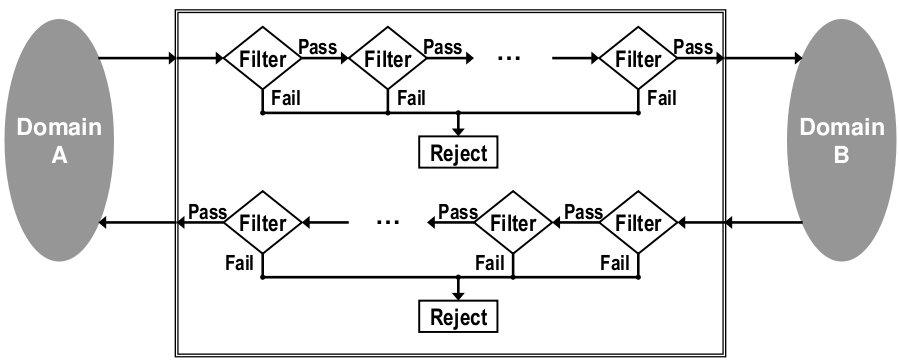
\includegraphics[width=5in]{nsa-legacy-arch}
\caption{NSA Legacy Notional Architecture Model}
\label{fig:model:conceptual-model}
\end{figure}

In the scenario portrayed in Figure \ref{fig:model:conceptual-model}, \textit{Domain A} could very well be a private cloud managed by the U.S. Air Force, while \textit{Domain B} is a public operational network of some kind shared by coalition partners in a joint operation.

A system user attempts to send a \textit{data package} consisting of a primary document and associated metadata from \textit{Domain A} to \textit{Domain B}.  At some point, that submission reaches a \textit{guard}, which contains at least one \textit{filter chain}.  Each filter chain then contains at least one \textit{filter}.  Individual filters can execute arbitrary actions over a submitted data package and have access to any number of external resources as required.  At any point, a filter can examine the data package and reject it, at which point it will frequently wait for human review.  If a filter does not reject a data package, it passes that package onto the next filter or submits it for delivery to Domain B.

\subsubsection{NSA, Services}
In recent years, the NSA has extended the legacy system architecture for cross-domain information sharing to exploit service-oriented computing styles \cite{proposal:nsa-arch}.  Visualized in Figure \ref{fig:model:conceptual-model-services}, this model incorporates more modern conceptual elements and componentry.

\begin{figure}[!t]
\centering
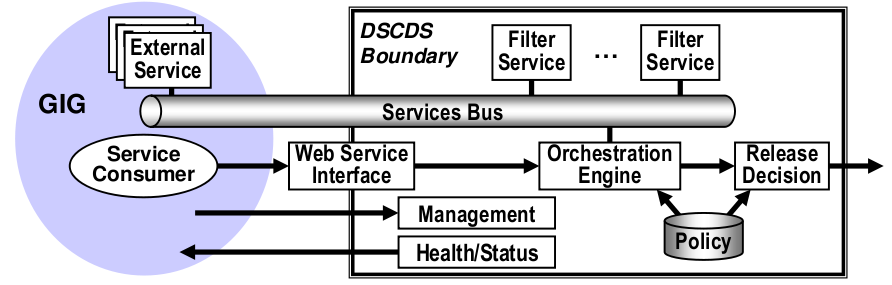
\includegraphics[width=5in]{nsa-arch}
\caption{NSA Service-Oriented Model}
\label{fig:model:conceptual-model-services}
\end{figure}

In the view in Figure \ref{fig:model:conceptual-model-services}, we see on the left the \textit{Global Information Grid}, or \textit{GIG}.  On the right, we have the \textit{Distributed Service-oriented Cross Domain Solution}, or \textit{DSCDS}.  The GIG is not a truly open system --- rather, it is a loosely coupled collection of computational services handing data at a variety of levels of sensitivity, federated to provide stakeholders timely access to relevant information \cite{proposal:gig-arch}.  The DSCDS is essentially the embodiment of the NSA's cross-domain vision applied to service oriented computing.  This model fuses various technology choices with previous cross-domain thinking.

Indicative of this more modern system design thinking, we have a variety of services and service consumers attached to a common service bus within the GIG.  Within the DSCDS, we have groups of filters implemented as services inspecting transferred data when moved over the bus.  Finally, all of this interaction is managed by a management interface and controlled by an orchestration engine accessing a centralized group of policies.

Note that here we have begun to access a common policy repository for various types of security metadata regarding primary data elements.

\subsubsection{Raytheon}
In the past few years, Raytheon has offered a new model for cross domain use influenced by the NSA service-oriented model \cite{proposal:raytheon-arch}.

\begin{figure}[!t]
\centering
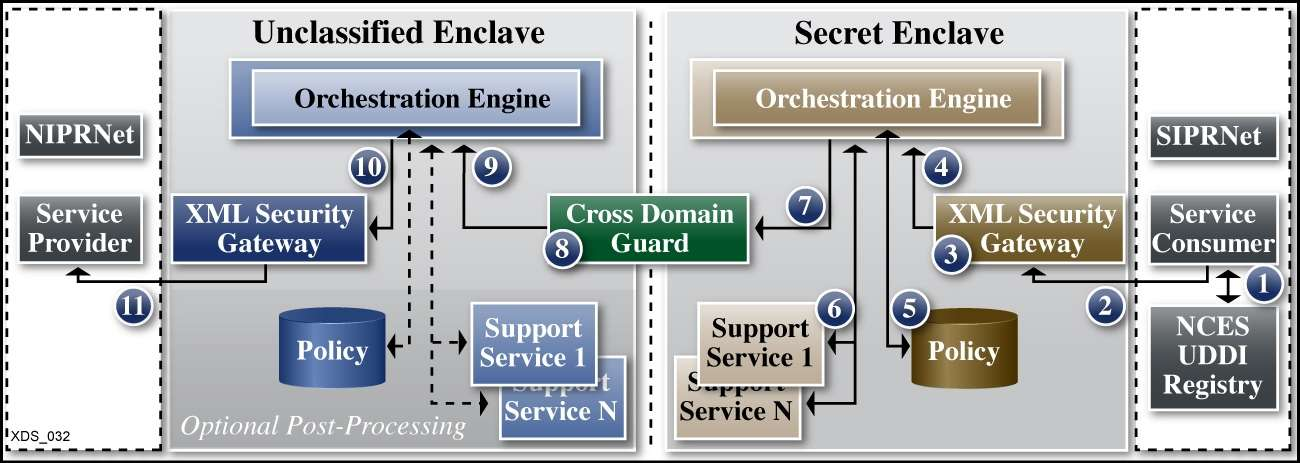
\includegraphics[width=5in]{raytheon-arch}
\caption{Ratheon Model}
\label{fig:model:conceptual-model-ray}
\end{figure}

The model in Figure \ref{fig:model:conceptual-model-ray}   is more grounded in the actual technical environment this kind of solution would be embedded within.  Here, we have the Non-secure Internet Protocol Router Network (NIPRNet) as one domain, and the Secret Internet Protocol Router Network (SIPRNet) as the other.  Here, NIPRNet is the lower security domain (lowside), and SIPRNet the higher security domain (highside).  This particular view shows the motion of data from the high side (SIPRNet) to the low side (NIPRNet).

Here, a data request is submitted from SIPRNet first two the \textit{XML Security Gateway} which calls into the \textit{Orchestration Engine} for policy validation.  The Orchstration Engine then coordinates calls into a \textit{Policy Repository} as well as to a collection of external \textit{Support Services}.  Once rectified against these elements, the request is passed into the \textit{Cross Domain Guard} which routes the request into the \textit{Unclassified Enclave} in NIPRNet.  Here, the request is passed directly through the lowside \textit{XML Security Gateway}, without rectification, onto the \textit{Service Provider}.  The response from the Service Provider is then passed back to the requester via the inverse path.

This model also begins to use a centralized policy repository, just as the NSA Service Model.  It also uses a single cross domain guard to transfer information from both the highside to the lowside, and vice-versa.

\subsubsection{Booz $\mid$ Allen $\mid$ Hamilton}
BAH submitted a competing model, also in 2009 \cite{proposal:bah-arch}.  In fact, both Raytheon and BAH presented their models under competitive contract to the UCDMO at the same conference, so the domain application is not coincidental.

\begin{figure}[!t]
\centering
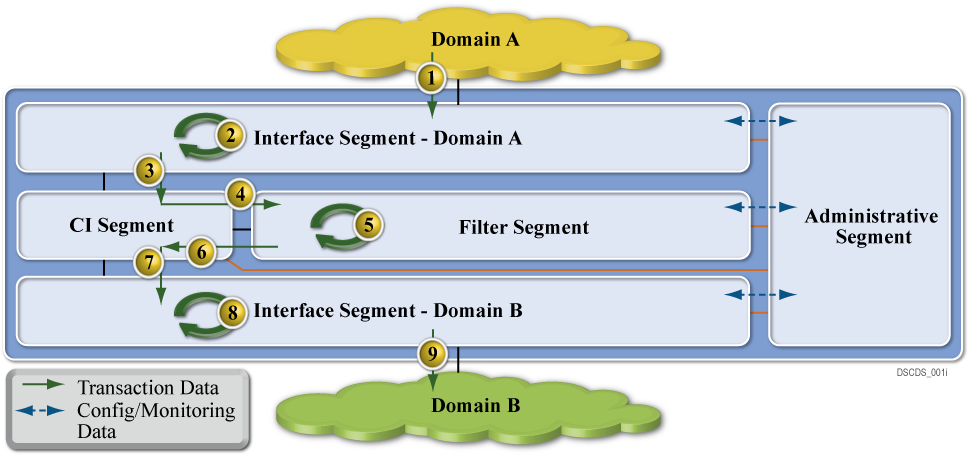
\includegraphics[width=5in]{bah-arch}
\caption{Booz | Allen | Hamilton Model}
\label{fig:model:conceptual-model-bah}
\end{figure}

Figure \ref{fig:model:conceptual-model-bah} embodies BAH's thinking with respect to cross domain information management.  We have a \textit{Domain A} as a high security domain, and \textit{Domain B} as a low security domain.  Here, we again have dataflow from the highside to the lowside through the cross domain management system.

While not as detailed as the Raytheon proposal, this does have similar elements.  Here, we data first travels from Domain A into the \textit{Interface Segment for Domain A}, similar to the secret enclave used in the Raytheon model.  From there, it moves into the \textit{CI Segment}, which in turn submits the transferring data into the \textit{Filter Segment}.  From there, the package is moved into the \textit{Interface Segment for Domain B}, and then onto \textit{Domain B}.  The \textit{Administrative Segment} provides managment and oversight of the system as a whole.

Note the absence of specific policy-centric elements.  This system is reliant on specific policy-agnostic content filters as well.

\subsubsection{Shortcomings of Current Systems}
Having reviewed the current state of the art of these kinds of cross domain solutions,  they still have clear similarities, and in fact have not progressed far beyond the initial notions of how these kinds of systems should work.  They still, for example, all use some kind of filter chaining mechanism to evaluate whether a given data item can be moved from a classified to an unclassified network.  Both NSA models used filters explicitly, as did the BAH model.  They all use a single guard as well, a sole point of security and enforcement, providing perimeter data security, but nothing else.  In each of these current system architectures, users are only allowed to exchange one type of information per domain.  The physical instantiations of these models are locked by operational policy to a single classification level limit.  Users cannot, for example, have Top Secret material on a network accredited for Secret material.  Finally, these models violate the end-to-end principle in large service network design, centralizing intelligence rather than pushing that intelligence down to the ends of the system \cite{Blumenthal:2001:RDI:383034.383037}.

\subsubsection{Characteristics of Future Systems}
Future systems will generally demonstrate decentralized policy management capabilities, infrastructural reuse, the ability to integrate with cloud systems, and security in depth.  Policy management is decentralized and integrated within the fabric of the system.  The system is both more secure and resilient as a result, better able to control information and operate under stressful conditions.  Multi-tenancy can lower costs and increase reliability and is furthermore a common attribute of cloud systems.  An appropriately secured system facilitates integration of computing resources into multi-tenant environments.  The ability to handle multi-tenant environments and to reliably secure both data at rest and data in motion leads to computational environments deployable in cloud systems.  Finally, systems must operate under \textit{all} conditions, including when they are under attack or compromise \cite{proposal:ron-ross}.  Ergo, they must provide protection to sensitive data in depth.

\subsection{Other Related Work}
This work introduces the notion of usage management embedded in a delivery network itself.  It also provides an in-depth analysis of the challenges and principles involved in the design of an open, interoperable usage management framework that operates over this kind of envrionment. Besides referencing the material we have covered in depth to portray the current state of the art, the analysis includes application of well-known principles of system design and standards~\cite{BlCl:01,Cl:88,ClWrSoBr:02}, research developments in the areas of usage control~\cite{PaSa:04,JaHeLa:10}, policy languages design principles~\cite{JaHeMa:06}, digital rights management (DRM) systems~\cite{JaHe:09},  and interoperability~\cite{JaHe:04,HeJa:05,KoLaMaMi:04,coral,marlin} towards the development of supporting frameworks.

While a large body of work exists on how overlay networks can use policies for \textit{network} management, very little work has been done on using usage policies for \textit{content} management.  The primary contribution in this area focuses on dividing a given system into specific \textit{security domains} which are governed by individual policies \cite{4457175}.  This system fits into our proposed taxonomy as an $\alpha$-type system as it has domains with single separating guards.

A large body of work currently exists with respect to security in and securing overlay networks.  These kinds of techniques and this area of study is vital to the production development and delivery of overlay systems, but is outside the scope of this work.

\section{Proposed Taxonomy}
A clear taxonomic organization of potential steps in approaching finer grained policy based usage management helps in describing the difficulties inherent in developing potential solutions as well as aiding in planning system evolution over time. Here, we have five distinct types of integrated policy-centric usage management systems, as shown in Table \ref{table:model:taxonomy}.  Of these five, only the first two levels are represented in current system model.

\begin{table}[tp] %
\centering %
\begin{tabular}{clcc}
\toprule %
$ Name$ 	& $Description$ \\\toprule %
$\phi$ 		& The initial level of this taxonomy, $\phi$ classified systems \\
 			& have a single guard without policy-based control \\\midrule
$\alpha$	& $\alpha$ classified systems have a single guard by have begun \\
			& to integrate policy-based control \\\midrule
$\beta$		& Systems that have begun to integrate policy-based control with \\
			& router elements are in the $\beta$ category \\\midrule
$\gamma$	& Systems that have integrated policy-based control with routing \\
			& and computational elements \\\midrule
$\delta$	& Continuous policy-based control with \textit{smart licensed} artifacts \\\bottomrule
\end{tabular}
\caption{Proposed Usage Management Taxonomy}
\label{table:model:taxonomy}
\end{table}

In this taxonomy, it is not required that systems pass through lower levels to reach higher ones.  This taxonomy represents a continuum of integration of usage management controls.  Systems can very well be designed to fit into higher taxonomic categories without addressing lower categories.  That said however, many of the supporting infrastructural services, like identification management or logging and tracing systems, are common between multiple levels.

The taxonomy itself starts with the current state, integrating policy evaluation systems into the network fabric gradually, moving away from filters, then by adding policy evaluation into the routing fabric, then the computational nodes, and finally by incorporating evaluation directly into content.

\subsection{$\phi$ --- Single Guard, No Policies}
The $\phi$ classification consists of systems like the initial NSA and BAH notional models in Figures \ref{fig:model:conceptual-model} and \ref{fig:model:conceptual-model-bah}.

\begin{figure}[!t]
\centering
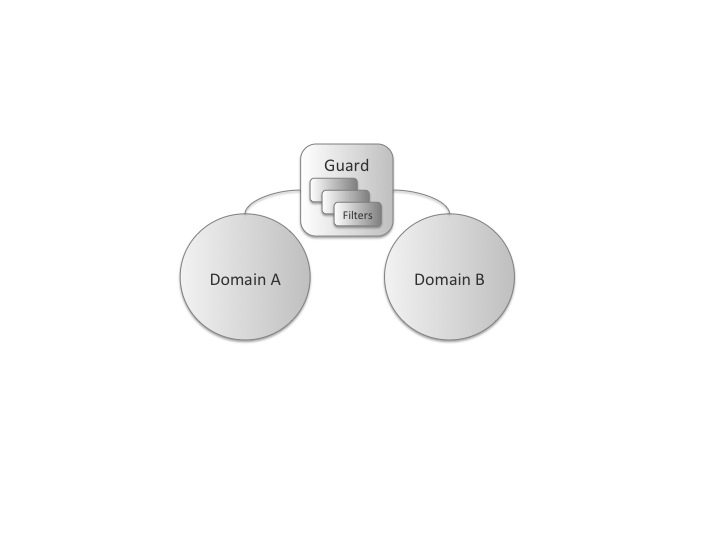
\includegraphics[width=5in]{model-phi}
\caption{Taxonomy ($\phi$)}
\label{fig:model:taxonomy-phi}
\end{figure}

These systems consist of two distinct domains, separated by a filter-centric single guard.  The initial NSA system model is clearly of this type, separating two domains with a guard using filter chains.  The BAH model is also of this type, using a Filter Segment to evaluate data packages transmitted between interface segments attached to specific domains.

Generally one of the domains supports more sensitive information than the other, but that is not always the case.  In the models we have examined this has certainly been true, but classified information for example  is commonly stored in \textit{compartments} which are separated by clear \textit{need-to-know} policies enforced by access lists and classification guides.  These kinds of compartments contain information at similar levels of classification, but contain distinct informational elements that should not be combined.

In these kinds of systems, specific rules regarding information transfer and domain characterization are tightly bound to individual filter implementations.

\subsection{$\alpha$ --- Single Guard, Policy Integration}
The $\alpha$ category begins to integrate policy-centric management rather than using strict content filtering.  The Raytheon model shown in Figure \ref{fig:model:conceptual-model-ray} and the service-oriented NSA model in Figure \ref{fig:model:conceptual-model-services} are $\alpha$ architectures as they both use policies to guide usage management decisions.

\begin{figure}[!t]
\centering
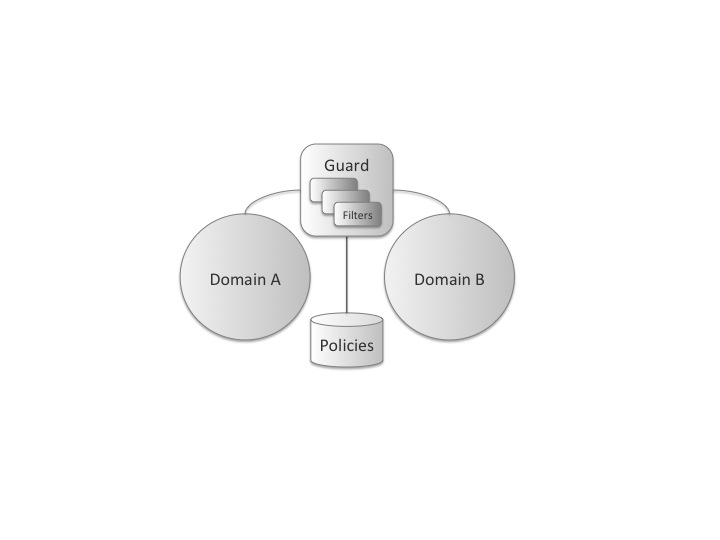
\includegraphics[width=5in]{model-alpha}
\caption{Taxonomy ($\alpha$)}
\label{fig:model:taxonomy-alpha}
\end{figure}

Here, we again have at least two domains, Domain A and Domain B, though we could potentially have more.  $\phi$ type systems require domain specific information to be tightly coupled to the filter implementations.  Separating the permissions, obligations, and other constraints from the filters and incorporating them into a specific separate policy entity frees the Guard from this coupling and provides additional flexibility to the system.

The guard can continue to use filters to process data.  These filters however are now more generic and decoupled from the specific domains it manages.  The choice of using a specific filtering model rather than some other kind of construct is a design detail level to implementers.  That said however, individual filters will be remarkably different and still need to understand the ontologies over which specific licenses are defined.

The policy repository is key to the implementation and differentiation of this taxonomy category.  This repository can be implemented as a separate repository keyed into via a data artifact's unique URI, for example.  It could also represent a policy sent in tandem with a data artifact in a data package.

The policy repository may be implemented as some kind of external service, and as such, represents the first such external service explicitly used in this taxonomy.  Other external services may well exist and be used to adjudicate information transfer decisions as well.

\subsection{$\beta$ --- Router Guards}
The $\beta$ taxonomic category begins to integrate policy-centric processing with router elements in a given network.  While this work is centered on using overlay technology to illustrate and implement these concepts, it is important to note that this kind of distributed policy-centric processing could very well be distributed into the physical routing fabric of a given network as well by extending Software Defined Networking systems like OpenFlow \cite{proposal:openflow}.

\begin{figure}[!t]
\centering
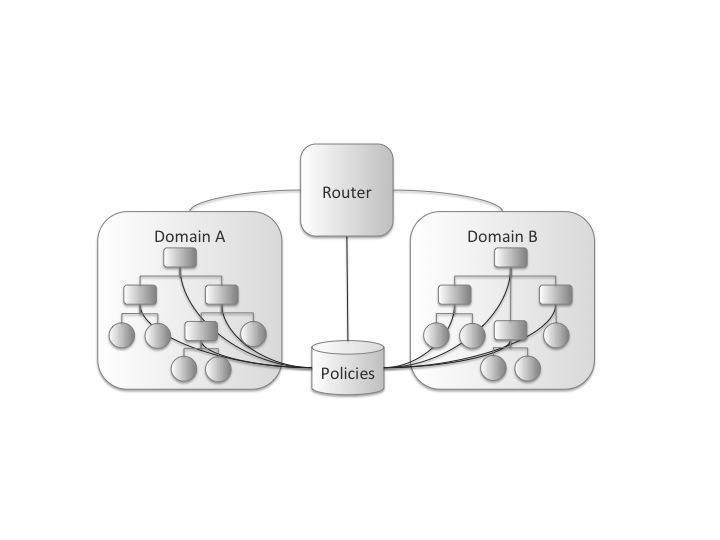
\includegraphics[width=5in]{model-beta}
\caption{Taxonomy ($\beta$)}
\label{fig:model:taxonomy-beta}
\end{figure}

In this model we can also host multiple domains as a result of flexible policy-based content examination.  Each domain hosts a network of some kind, though that hosted network could very well be a degenerate network of a single system.  Each network hosted in a domain is hierarchical, with specific computational nodes embodied by workstations, tablet computers or mobile devices, and routing points embodied by routers or switches of some kind.

Policy evaluation in this model has begun to penetrate into the routing elements of the specific domain networks.  Here, note that we have started to penetrate into the routing fabric of the network by doing content evaluation at router points.  Content-based switching networks have been successful in other domains, and such techniques can be used here to provide policy evaluation capabilities.  

Certain types of traffic are easier to evaluate than others however.  For example, HTTP requests and responses are easier to examine that TCP packets.  When examining TCP packets, systems generally require additional context to select an appropriate packet window (e.g. the number of packets cached for examination).  HTTP traffic does not usually require this kind of flexibility.

This migration of policy evaluation into the routing fabric provides for enhanced data security and better network management, especially if part of a network is compromised.  Now that policy decisions can be made at the router level in a given network, we are starting to have network security in depth rather than simple perimeter protection.  This not only provides the ability for additional information protection, but also allows for different compartments holding information at different need-to-know levels to be created ad-hoc under different routing segments.  In cases of network compromise, this kind of dynamic policy enforcement can also allow for quick node excision as well.

\subsection{$\gamma$ ---  Router and Node Guards}
The $\gamma$ compartment has integrated policy evaluation with compute and routing nodes.  Here, policies can be evaluated against content at all network levels --- nodes emitting requests, nodes fielding requests, and all routing elements in between.

\begin{figure}[!t]
\centering
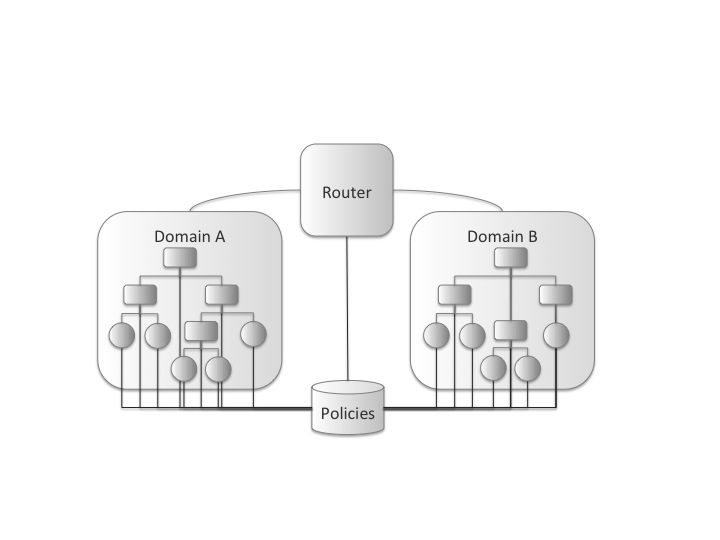
\includegraphics[width=5in]{model-gamma}
\caption{Taxonomy ($\gamma$)}
\label{fig:model:taxonomy-gamma}
\end{figure}

In Figure \ref{fig:model:taxonomy-gamma}, we see that the policy repository is supplying services to all computational elements in both domains.  This gives us increased granularity with respect to data compartmentalization by integrating information security into each network element.  At this point, the network can create compartments of single nodes, while previously in $\beta$ level systems compartments could only be created under specific routing elements.  At this level, we can also provide services revoking data access based on policy evaluation decisions when needed.

Furthermore, individual node exclusion is possible as well. $\beta$ classified systems could excise network elements under specific routers by dynamic policy application.  Now, we can apply the same functionality to individual compute nodes.  For example, if a networked device like a smart phone is compromised, that device can be removed from access quickly or used to feed mis-information to adversaries.

\subsection{$\delta$ --- Continuous Evaluation}
At this level of the taxonomy, we are not passing data packages around which we then examine and make judgments against.  Rather, we now have a system based around a \textit{smart license} where decisions regarding use and routing are asked of the data package itself.

Smart licenses simplify the deployment environment.  They are essentially packages of mobile code, and as such require an environment in which to run but that environment does not need to support all the system elements that it would otherwise need to integrate.  Usage history, management decisions, policy evaluation, and other components would be packaged into this smart license and distributed.  Hosts would need to provide the appropriate environment in which these licenses run, but little else.

These kinds of licenses are able to manage dynamic context more effectively.  As usage history accompanies each smart license, such usage no longer needs to be managed by an external service. Furthermore, offline use is much easier to implement as much of the information is omnipresent in the smart license package.

The cost for these advantages is additional license development complexity.  The license needs to support offline use via some kind of caching mechanism and needs to be able to interact with the local environment as well as the larger enterprise environment.  It is no longer a data-centric package of artifacts and meta-data, but is rather an actual program moving through various systems of the network.

\section{Scope and Contribution of Work}
The unique contribution of this work is a quantitative analysis of policy-centric overlay network options, associated taxonomies of use, and prototypical technology proofs-of-concept.  This work wil use overlay network approaches with semantic web  technology to prototype example systems.  The process of examining and developing this area of knowledge will specifically address:

\begin{itemize}
\item \textit{Overlay Options} --- This includes various types of overlay networks and associated strengths and weaknesses addressing centralized and decentralized models.  Here, this work will produce detailed quality attribute-centric architectural analysis specifically addressing confidentiality, integrity, and availability, examining both structured and unstructured overlay approaches.
\item \textit{Taxonomies of Use} --- Depending on the specific usage management requirements and context, different overlays have different applicability; this work will provide guidance on suitability by more completely developing the taxonomy of policy integration presented herein.
\item \textit{Prototypical Technologies} --- Examples and proofs-of-concept will be required to appropriately analyse various architectural alternatives.  The course of this work will develop both structured and unstructured systems demonstrating and validating the overlay taxonomy, collecting experimental results from these prototypical systems with respect to identified system quality attributes for analysis to support architectural expectations.
\end{itemize}

This work will focus on the $\alpha$, $\beta$, and $\gamma$ taxonomic categories, excluding $\delta$ and $\phi$ classed systems.

\newpage

\bibliographystyle{plain}
\bibliography{bib/proposal,bib/drm}

\end{document}